\setchapterstyle{lines}
\chapter{FESTIM verification}\label{appendix verification}

\section{Conservation of chemical potential (MES)}
This verification case aims at checking the FESTIM code is correctly solving the governing \refeq{c/s conservation}, Equation \ref{eq:mobile} and \ref{eq: diffusion equation changed}.

\begin{figure*} [h]
    \centering
    \begin{subfigure}{0.5\linewidth}
        \centering
        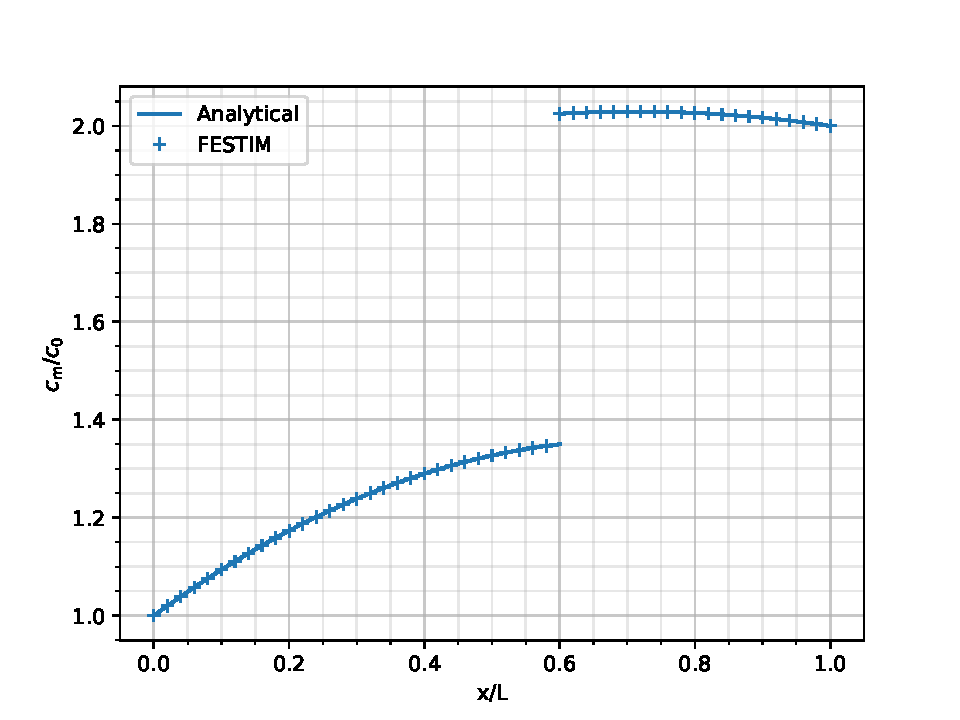
\includegraphics[width=\linewidth]{Figures/Chapter3/monoblocks/interface_condition/out_MES_case1.pdf}
        \caption{Case 1: $\alpha = 2$, $\beta = 1.5$, $\gamma=0.6$, $\tilde{c}_L = 2$, $\tilde{f}=1$.}
    \end{subfigure}%
    % \hfill
    \begin{subfigure}{0.5\linewidth}
        \centering
        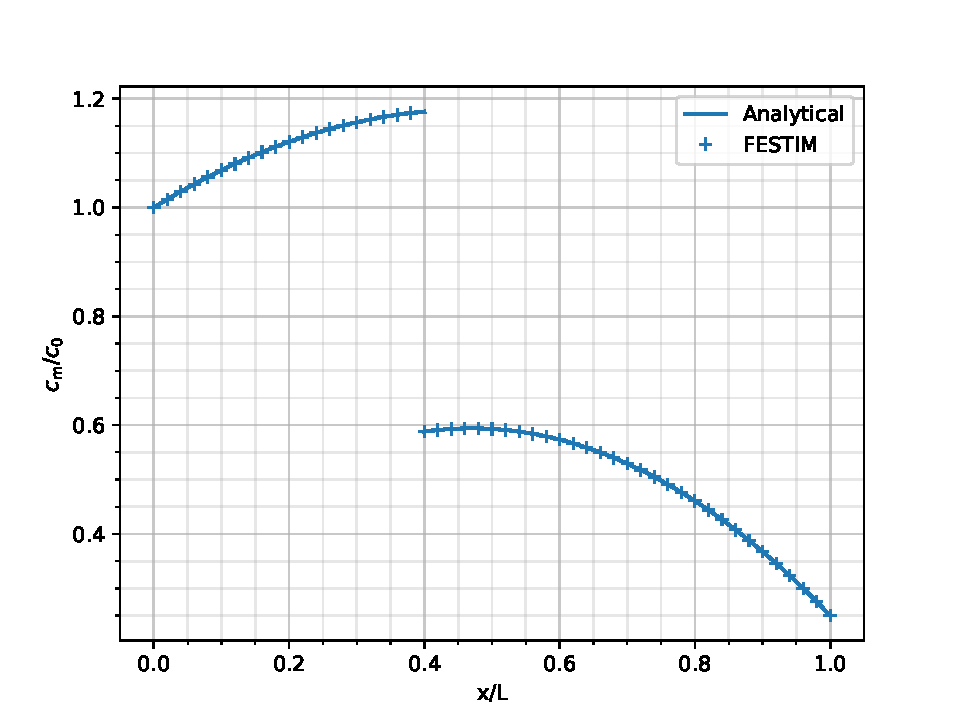
\includegraphics[width=\linewidth]{Figures/Chapter3/monoblocks/interface_condition/out_MES_case2.pdf}
        \caption{Case 2:  $\alpha = 1.5$, $\beta = 0.5$, $\gamma=0.4$, $\tilde{c}_L = 0.25$, $\tilde{f}=2$.}
    \end{subfigure}
    \caption{Concentration profiles simulated by FESTIM against analytical solutions.}
    \label{fig:comparison MES}
\end{figure*}

The uni-dimensional test case considered in this Section was made of two subdomains $\Omega_1$ and $\Omega_2$ and is described as follow:
\begin{subequations}
\begin{align}
    \Omega &= [0, L] = \Omega_1 \cup \Omega_2 \\
    \Omega_1 &= [0, x_\mathrm{int}] \\
    \Omega_2 &= [x_\mathrm{int}, L] \\
    D &= \begin{cases}
        D_1,& \text{ in } \Omega_1\\
        D_2,& \text{ in } \Omega_2
    \end{cases} \\
    S &= \begin{cases}
        S_1,& \text{ in } \Omega_1\\
        S_2,& \text{ in } \Omega_2
    \end{cases}
\end{align}
\end{subequations}

The following dimensionless quantities are introduced:
\begin{subequations}
    \begin{align}
        \tilde{c}_\mathrm{m} &= c_\mathrm{m} / c_0\\
        \tilde{x} &= x / L \\
        \tilde{f} &= f \frac{L^2}{D_\mathrm{eq} c_0} \\
        \alpha &= D_2/D_1 \\
        \beta &= S_2/S_1 \\
        \gamma &= x_\mathrm{int}/L\\
    \end{align} 
\end{subequations}
where $D_\mathrm{eq} = (D_1 D_2)^{1/2}$.

By integrating Equation \ref{eq:mobile} and assuming steady-state (i.e.\ $\partial c/\partial t=0$), one can obtain the following dimensionless form:

\begin{equation}
        \tilde{c}_\mathrm{m}= 
\begin{cases}
    -\frac{1}{2}\alpha^{1/2}\tilde{f} \tilde{x}^2 + a_1 \tilde{x} + b_1,& \text{ in } \Omega_1\\
    -\frac{1}{2}\alpha^{-1/2}\tilde{f} \tilde{x}^2 + a_2 \tilde{x} + b_2,& \text{ in } \Omega_2
\end{cases}
\label{eq:MES c}
\end{equation}

where $a_1$, $b_1$, $a_2$, $b_2$ are the unknowns of the problem to be determined.
The boundary conditions and the equilibrium law at the interface are defined as:
\begin{subequations} \label{eq: bcs MES}
\begin{align} 
        \tilde{c}_\mathrm{m}(\tilde{x}=0) & = 1 \\
        \tilde{c}_\mathrm{m}(\tilde{x}=1) & =  \tilde{c}_L \\
        \tilde{c}_\mathrm{m}^-(\tilde{x}=\gamma) & =  \beta \; \tilde{c}_\mathrm{m}^+(\tilde{x}=\gamma)\\
        \nabla \tilde{c}_\mathrm{m}^-(\tilde{x}=\gamma) & =  \alpha \nabla \tilde{c}_\mathrm{m}^+(\tilde{x}=\gamma)
\end{align}
\end{subequations}


Equation \ref{eq:MES c} can be solved with these constraints and coefficients describing $\tilde{c_\mathrm{m}}$ therefore read:

\begin{align}
    \begin{split}
        a_1 &= a_0 \; \alpha^{1/2}  \\
        b_1 &= 1 \\
        a_2 &= a_0 \; \alpha^{-1/2}\\
        b_2 &= \tilde{c}_L + \frac{1}{2} \alpha^{-1/2} \tilde{f} - a_2 \\
        a_0 &= \frac{2 \alpha^{1/2}( \tilde{c}_L - \beta) + \tilde{f}  (\gamma^{2} \left(\alpha \beta - 1\right) + 1)}{1  - \gamma + \alpha \beta \gamma} \\
    \end{split}
    \label{eq: MES c coefficients}
\end{align}

It is worth noting that when $\beta=1$ (i.e.\ $S_1 = S_2 = S$) the solution becomes independent of $S$ and {$c_\mathrm{m}^{-}(x_\mathrm{int}) = c_\mathrm{m}^{+}(x_\mathrm{int})$}.
Moreover, when $\alpha = 1$ (i.e.\ $D_1 = D_2 = D$), then $a_1 = a_2 = a_0$ which is the solution for steady-state diffusion in a mono-material.

The solution computed by FESTIM was found to be in very good agreement with the analytical solution for several test cases (see Figure \ref{fig:comparison MES}).

 
However, this method does not exercise all the terms in the governing Equation \ref{eq: diffusion equation changed}.
For instance, this analytical solution is only uni-dimensional, steady state is assumed and material properties are constant within the materials.
Having an exact solution from an analytical resolution for a general problem (multidimensional, transient, heterogeneous material properties, etc...) is often complex.
In order to exercise all these terms, the Method of Manufactured Solutions (MMS) will therefore be employed for it offers a good alternative to unravel these complexities.

\section{Conservation of chemical potential (MMS)}

This verification case aims at checking the FESTIM code is correctly solving the governing \refeq{c/s conservation}, Equation \ref{eq:mobile} and \ref{eq: diffusion equation changed}.

The domain $\Omega$ for this test problem is a unit square composed of two subdomains $\Omega_1$ and $\Omega_2$ (see Equation \ref{eq: MMS domain}).
\begin{subequations} \label{eq: MMS domain}
\begin{align}
    \Omega &= [0, 1] \times [0, 1] \\
    \Omega_1 &= [0, x_\mathrm{int}] \times [0, 1] \\
    \Omega_2 &= [x_\mathrm{int}, 1] \times [0, 1] \\
\end{align}
\end{subequations}
In order to unravel the complexity of an analytical resolution of the direct problem, a manufactured solution $c_\mathrm{m}$ was constructed (see Equation \ref{eq: manufactured solution}) and the problem was solved backwards.

\begin{equation}
        c_M= 
\begin{cases}
    c_{M1},& \text{ on } \Omega_1\\
    \frac{S_2}{S_1} \cdot c_{M1},& \text{ on } \Omega_2
\end{cases}
\label{eq: manufactured solution}
\end{equation}
where $c_{M1} = 2 + \cos(2\pi x) \cdot \cos(2\pi y) + t$

It is worth noting that, when choosing a manufactured solution, one must ensure it satisfies all the governing equations (especially \refeq{c/s conservation}).
In our case, $c_M$ ensures the flux conservation at the interface and the continuity of the quantity $c_\mathrm{m}/S$.

Properties are assumed time and space dependent in order to test every portion of the code (see Equation \ref{eq: MMS properties}).
\begin{subequations}
    \begin{align}
        D_1(x, y, t) & =  D_{1_0} \exp(-E_{D_1}/(k_B \cdot T(x,y, t) )) \\
        D_2(x, y, t) & =  D_{2_0} \exp(-E_{D_2}/(k_B \cdot T(x,y, t) )) \\
        S_1(x, y, t) & =  S_{1_0} \exp(-E_{S_1}/(k_B \cdot T(x,y, t) )) \\
        S_2(x, y, t) & =  S_{2_0} \exp(-E_{S_2}/(k_B \cdot T(x,y, t) )) \\
        T(x, y, t) & = 500 + 30 \cos(2\pi x) \cos(2 \pi y) \cos(2 \pi t)
\end{align} \label{eq: MMS properties}
\end{subequations}
with ${k_B = \SI{8.617e-5}{eV.K^{-1}}}$ the Boltzmann constant, $D_{1_0} = 1$, $E_{D_1} = 0.1$, $D_{2_0} = 2$, $E_{D_2} = 0.2$, $S_{1_0} = 1$, $E_{S_1} = 0.1$, $S_{2_0} = 2$ and $E_{S_2} = 0.2$.
The temperature $T$ varies around \SI{500}{K} so that, given the activation energies, properties do not approach zero.

By injecting the manufactured solution $c_M$ into the governing Equation \ref{eq:mobile}, the source term can be expressed as:
\begin{align}
    f(x, y, t) &= \frac{\partial c_M}{\partial t} - \vec{\nabla} \cdot\left(D(x, y)
    \vec{\nabla}c_M\right) \nonumber \\
    &= \begin{cases}
        \frac{\partial c_{M_1}}{\partial t} - \vec{\nabla} \cdot\left(D_1(x, y)
    \vec{\nabla}c_{M_1}\right),& \text{ on } \Omega_1\\
    \frac{\partial c_{M_2}}{\partial t} - \vec{\nabla} \cdot\left(D_2(x, y)
    \vec{\nabla}c_{M_2}\right),& \text{ on } \Omega_2\\
    \end{cases}
\end{align}

The source term $f$ was then fed into FESTIM alongside with the initial and boundary conditions described below:
\begin{subequations}
    \begin{align}
        c_\mathrm{m}(x, y, t) &= c_M(x, y, t), \text{ on } \partial \Omega \\
        c_\mathrm{m}(x, y, t=0) &= c_M(x, y, t=0), \text{ on } \Omega
    \end{align}
\end{subequations}

The computed solution $c_\mathrm{comp}$ can then be compared with the manufactured solution $c_M$ in order to quantitatively measure the numerical error.
After running the MMS process, the computed solution and the manufactured solution were in very good agreement at several arbitrarily chosen times of simulation (see Figure \ref{fig: results MMS}).
% The stepsize was $\Delta t=0.01$.
The absolute difference between the manufactured solution and the computed one was found to be zero on the boundary and maximum at the interface between the two materials.
This is explained by the Dirichlet boundary conditions enforcing the computed solution on the boundary.
This difference decreases by increasing the mesh refinement and decreasing the stepsize.
Nonetheless, the error was found to remain orders of magnitude lower than the actual solution.

\begin{figure*}
    \centering
    \begin{subfigure}{0.33\linewidth}
        \centering
        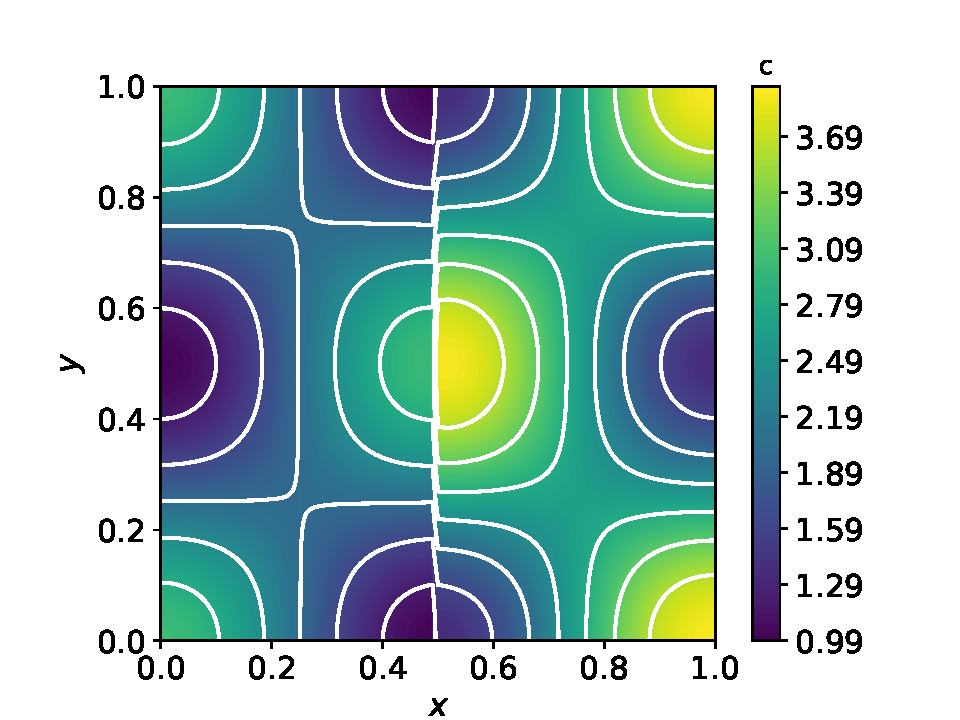
\includegraphics[width=\linewidth]{Figures/Chapter3/monoblocks/interface_condition/u_computed_t0.01.pdf}
        \caption{Computed solution $c_\mathrm{comp}(t=0.01)$.}
    \end{subfigure}%
    \begin{subfigure}{0.33\linewidth}
        \centering
        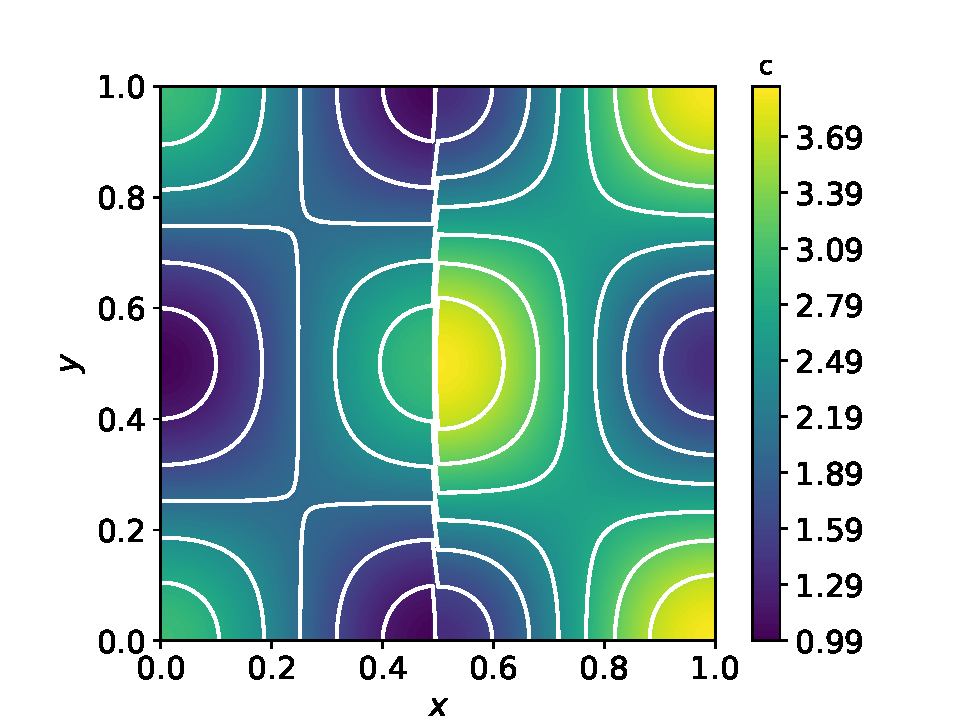
\includegraphics[width=\linewidth]{Figures/Chapter3/monoblocks/interface_condition/u_exact_t0.01.pdf}
        \caption{Exact solution $c_M(t=0.01)$.}
    \end{subfigure}%
    \begin{subfigure}{0.33\linewidth}
        \centering
        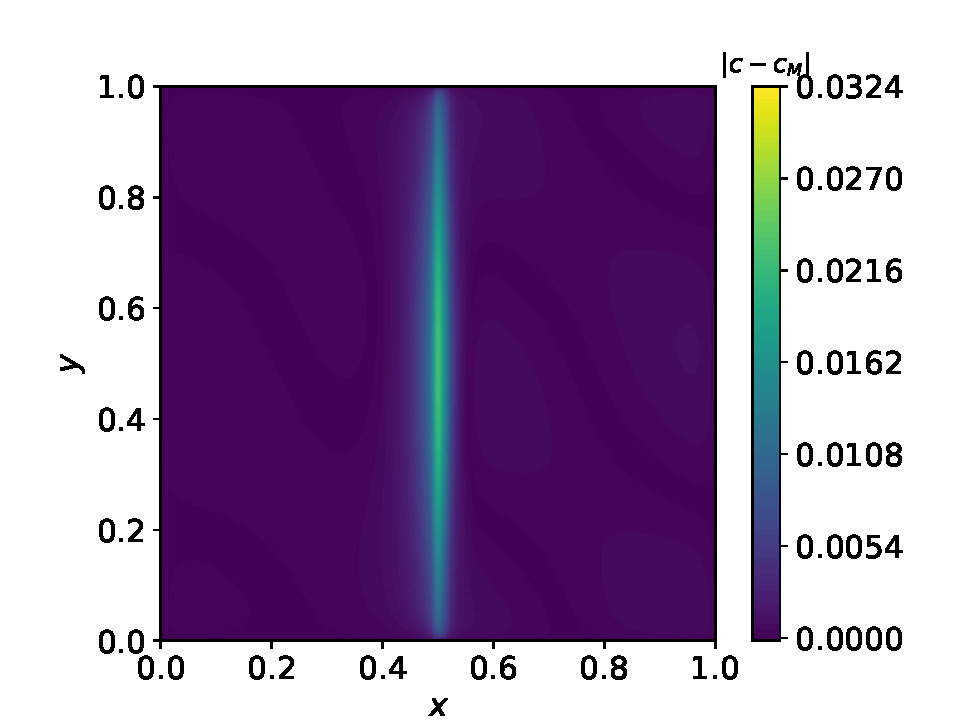
\includegraphics[width=\linewidth]{Figures/Chapter3/monoblocks/interface_condition/diff_t0.01.pdf}
        \caption{Absolute difference.}
    \end{subfigure}
    \begin{subfigure}{0.33\linewidth}
        \centering
        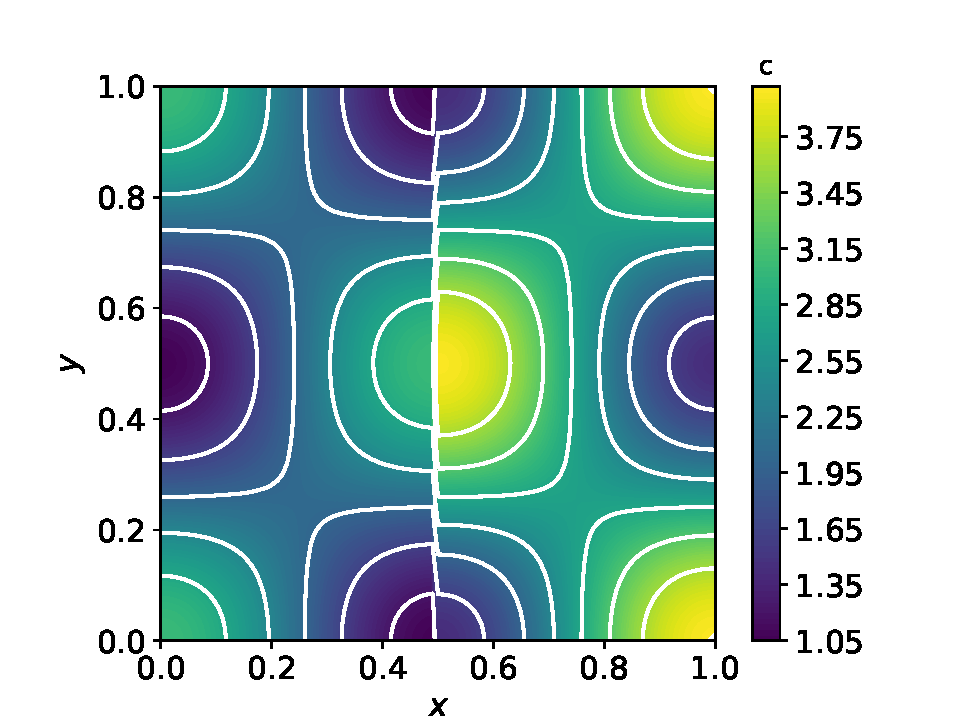
\includegraphics[width=\linewidth]{Figures/Chapter3/monoblocks/interface_condition/u_computed_t0.06.pdf}
        \caption{Computed solution $c_\mathrm{comp}(t=0.06)$.}
    \end{subfigure}%
    \begin{subfigure}{0.33\linewidth}
        \centering
        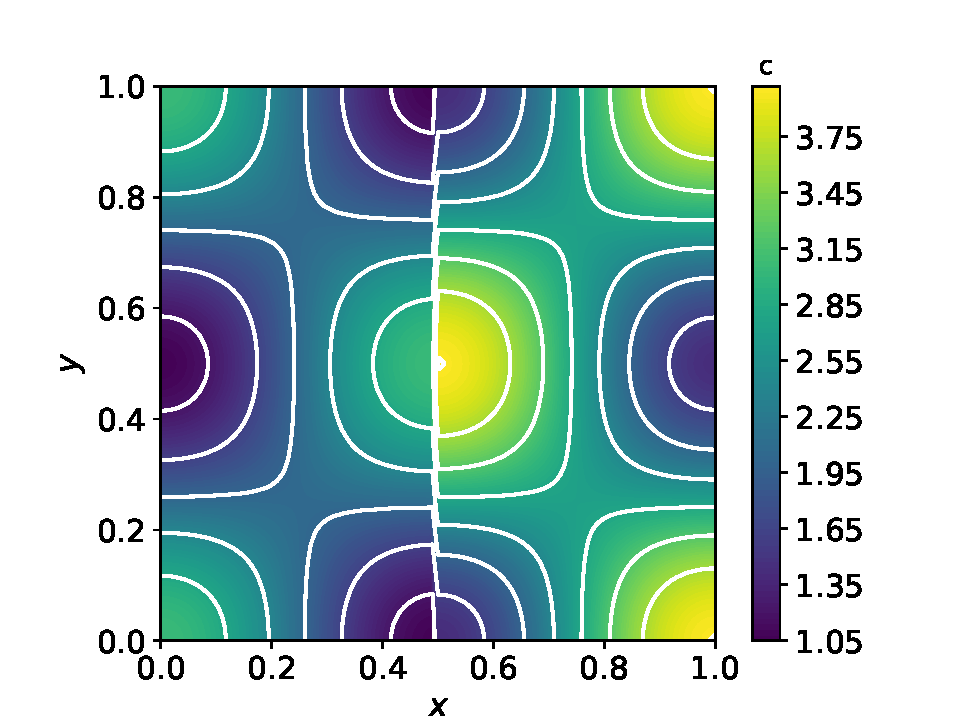
\includegraphics[width=\linewidth]{Figures/Chapter3/monoblocks/interface_condition/u_exact_t0.06.pdf}
        \caption{Exact solution $c_M(t=0.06)$.}
    \end{subfigure}%
    \begin{subfigure}{0.33\linewidth}
        \centering
        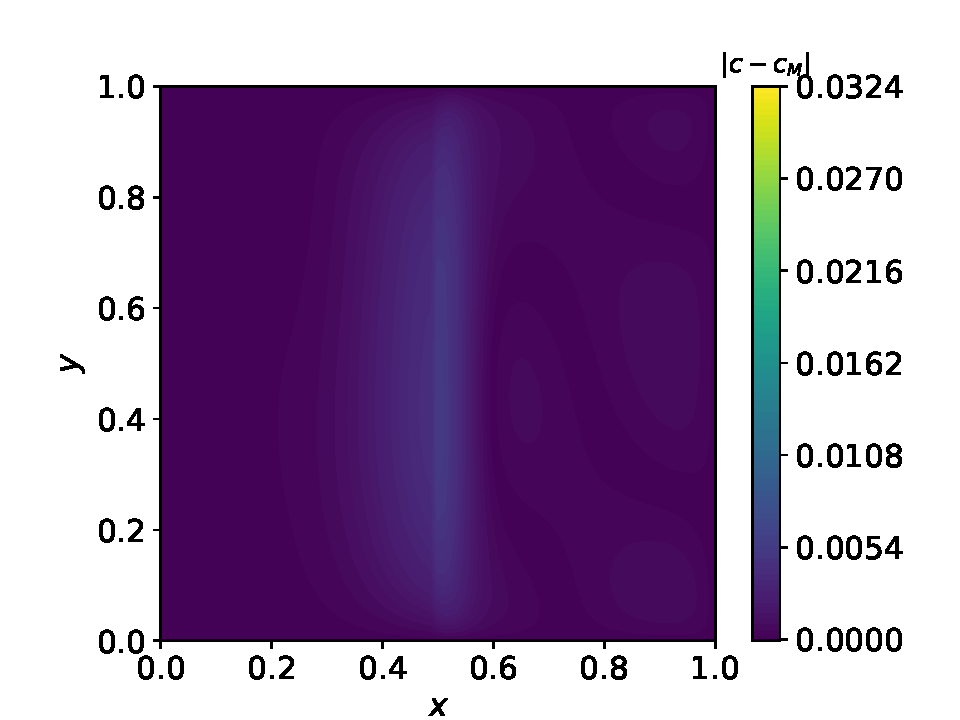
\includegraphics[width=\linewidth]{Figures/Chapter3/monoblocks/interface_condition/diff_t0.06.pdf}
        \caption{Absolute difference.}
    \end{subfigure}
    \caption{Comparison of concentration fields simulated by FESTIM with manufactured solutions.}
    \label{fig: results MMS}
\end{figure*}


\section{Heat transfer (MMS)}

% why not use a complex geometry? like an elbow

The heat transfer module in FESTIM can also be verified using the method of manufactured solutions.

Let us choose the following test problem on a elbow domain $\Omega = [0, 1] \times [0, 0.5] \cup [0, 0.5] \times [0.5, 1]$ with the manufactured solution $T_D(x, y) = \sin(\omega \pi x) \sin(\omega \pi y)$.

\begin{align}
    \nabla \cdot \lambda \nabla T &= -f \\
    T &= T_D \text{  on  } y \in [0, 1] \\
    -\lambda \nabla T \cdot \mathbf{n} &= -\lambda \nabla T_D \cdot \mathbf{n} \text{  on  other surfaces} \\
    \lambda(x, y) &= 2 + T_D^2 \\
\end{align}

The source term $f$ is therefore:
\begin{align}
    f &= 2 \pi^{2} \omega^{2} f_0 \sin{\left (\pi \omega x \right )} \sin{\left (\pi \omega y \right )} \\
    f_0 &= \left(3 f_1 f_2 - f_1 - f_2 + 2\right) \\
    f_1 &= \sin^{2}{\left (\pi \omega x \right )} \\
    f_2 &= \sin^{2}{\left (\pi \omega y \right )} \\
\end{align}

The computed FESTIM solution is extremely similar to the exact solution (see Figure \ref{fig: results MMS heat transfer}).
It is also possible to compute the L2-error for several number of cell divisions in the x and y directions $N$ to ensure the error decreases as a power law of $N$.
Moreover, the L2-error should be proportional to $h^{d+1}$ where $h=1/N$ and $d$ is the polynomial degree of the elements \sidecite{vu-huu_convergence_2021}.
This was verified for \gls{p1} and \gls{p3} elements and a super-convergence rate was observed for the \gls{p2} elements (see Figure \ref{fig: convergence rates heat transfer}).

\begin{figure*}
    \centering
    \begin{subfigure}{0.5\linewidth}
        \centering
        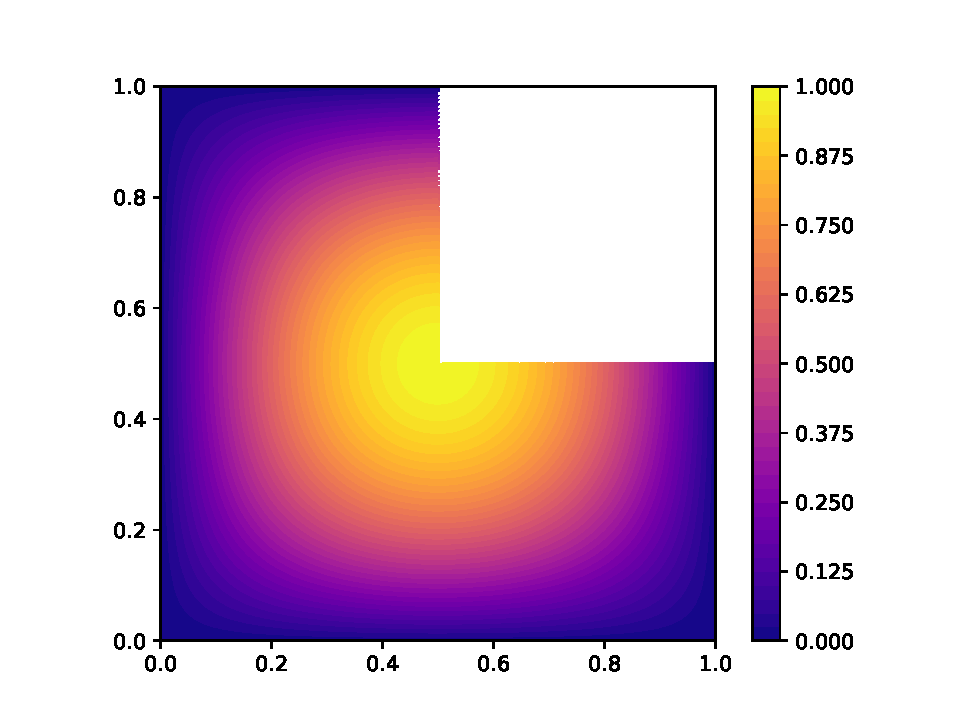
\includegraphics[width=\linewidth]{Figures/Chapter2/T.pdf}
        \caption{Computed temperature $N=64$.}
    \end{subfigure}%
    \begin{subfigure}{0.5\linewidth}
        \centering
        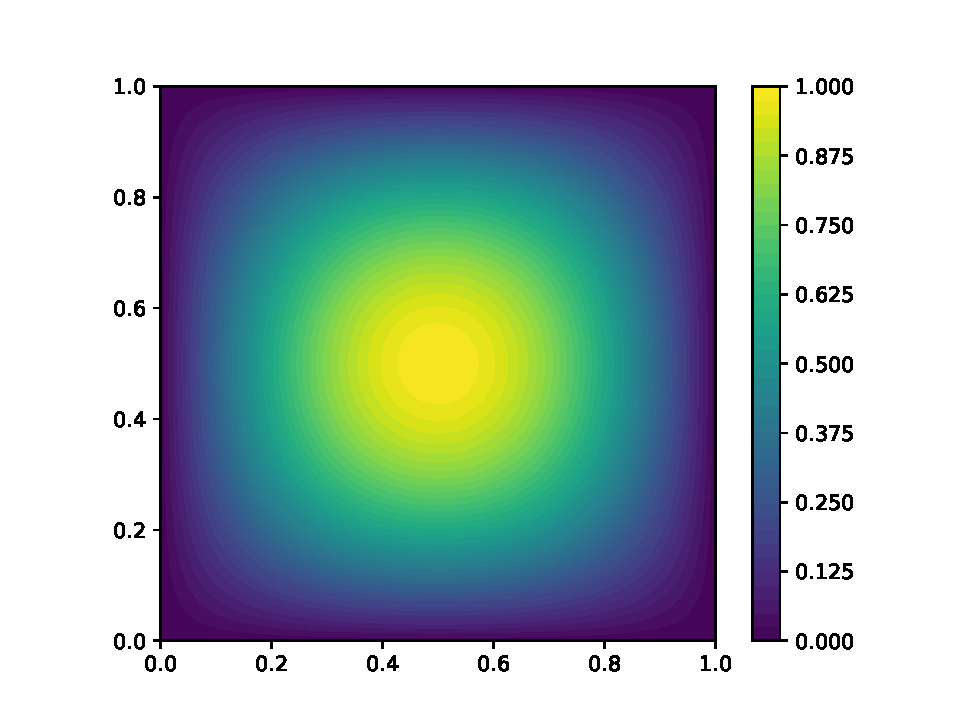
\includegraphics[width=\linewidth]{Figures/Chapter2/T_exact.pdf}
        \caption{Exact temperature.}
    \end{subfigure}

    \caption{Verification of the heat transfer module in FESTIM.}
    \label{fig: results MMS heat transfer}
\end{figure*}

\begin{figure}
    \centering
    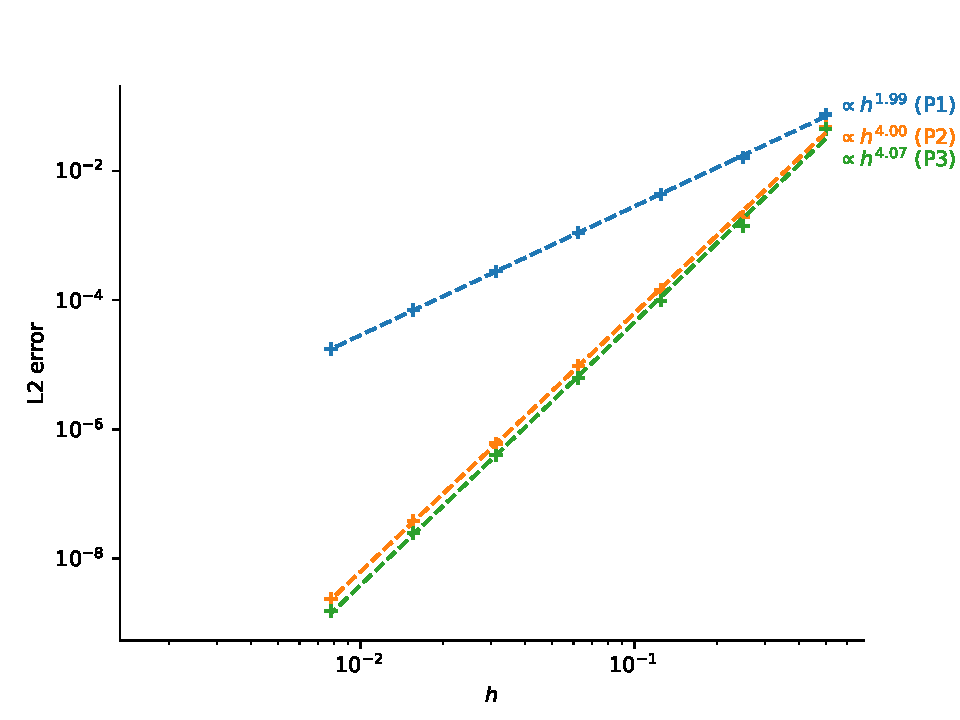
\includegraphics[width=\linewidth]{Figures/Chapter2/convergence_rate_heat_transfer.pdf}
    \caption{Evolution of the L2 error on $T$ showing the convergence rates for the 2D heat transfer case.}
    \label{fig: convergence rates heat transfer}
\end{figure}
